\section{Methodology}\label{sec:Methodology}

The methodology used in this research is summarized in the flowchart in \textbf{Figure \ref{fig:CH03_Methodology}}. 

\begin{figure}[h]
    \centering
    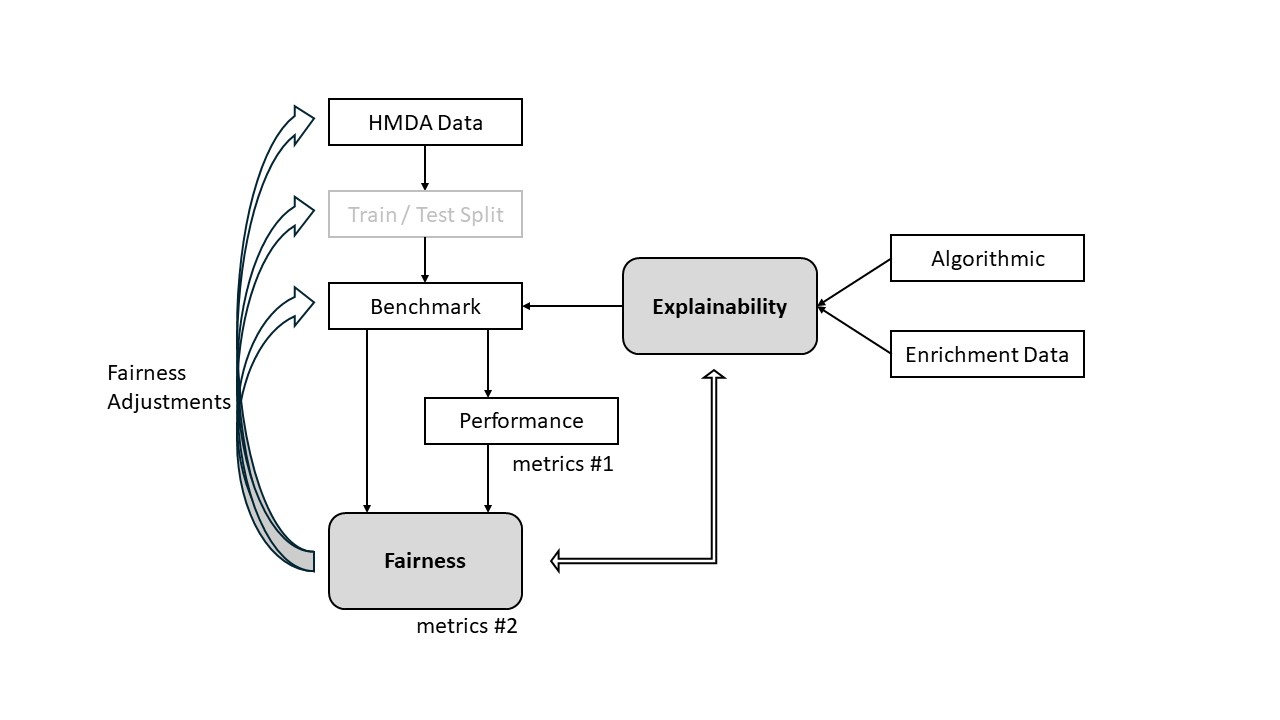
\includegraphics[width=0.85\textwidth]{CH03_Methodology.jpg}
    \caption{Methodology}
    \label{fig:CH03_Methodology}
\end{figure}

Data Preparation and Splitting have already been discussed in \textbf{Chapter \ref{subsec:Data_Preparation}}, details on the remaining steps will be provided in the following.

\subsection{Model Training and Prediction}\label{subsec:Model_Training_and_Prediction}

The model chosen is a comparably simple sequential neural network, implemented with the keras package. Model details are provided in \textbf{Table \ref{tab:CH03_Model_Details}}.

\begin{table}[h]
    \centering
    \begin{tabularx}{\textwidth}{lXr}
    \hline
    \textbf{Layer (type)} & \textbf{Output Shape} & \textbf{Param \#} \\
    \hline
    dense & (None, 32) & 640 \\
    dense\_1 & (None, 64) & 2112 \\
    dropout & (None, 64) & 0 \\
    dense\_2 & (None, 128) & 8320 \\
    dropout\_1 & (None, 128) & 0 \\
    dense\_3 & (None, 64) & 8256 \\
    dropout\_2 & (None, 64) & 0 \\
    dense\_4 & (None, 1) & 65 \\
    \hline
    \textbf{Total params} & & 19,393 \\
    \textbf{Trainable params} & & 19,393 \\
    \textbf{Non-trainable params} & & 0 \\
    \hline
    \end{tabularx}
    \caption{Summary of the Neural Network}
    \label{tab:CH03_Model_Details}
\end{table}

To increase the efficiency of the training process and to prevent overfitting, \textit{callbacks} for early stopping (with a patience of 5 iterations) and best model selection, both based on the validation loss, have been implemented. 
\textit{Adam} is chosen as the optimizer, due to the nature of the classification task, loss evaluation is based on \textit{binary crossentropy}, and \textit{accuracy} is selected as the target metric. Training takes place with a batch size of 48 and for a maximum of 30 epochs. 

\subsection{Explainability}\label{subsec:Explainability}

% Algorithm choice: Choice of model, reasoning, details of application
% Comment on SHAP and LIME disagreement and add https://arxiv.org/pdf/2202.01602.pdf
% Enrichment data: Explain use of geographical detail 



\subsection{Performance Assessment}\label{subsec:Performance_Assessment}

The model originally puts out numerical probabilities, which are then converted to binary values, using a threshold of 0.5.
Using these original probabilities, \textbf{ROC AUC} curves can be plotted and the ROC AUC score can be calculated, which is used as one of the assessment measures.
Additionally, a common set of classification metrics, being \textbf{accuracy}, \textbf{precision}, \textbf{recall}, and \textbf{F1 score}, are calculated alongside the \textbf{confusion matrix}.

Finding comparable benchmarks for model performance in the academic literature is hampered by the recency of the used data and the individual approach to filtering states.
Papers with a similar approach were able to achieve a ROC AUC of \textit{0.768} on a regression task \parencite{Ghoba} with somewhat comparable data, 
or reported an accuracy of 91\% using a deep neural network for classification \parencite{Hodges2024}, albeit with a different timeframe and a higher amount of used features. 

\subsection{Fairness Assessment}\label{subsec:Fairness_Assessment}

% Describe aequitas procedure
% Describe aif360 procedure(?)
% Refer to formulas from literature review (and probably move / delete them)
% Metrics: Choice of metrics, reasoning, details of application - choose most important ones from aequitas summary

Aequitas provides a multitude of fairness metrics to provide model fairness. In order to work with a uniform framework in this thesis, four easy to understand yet highly relevant metrics are chosen: 
The disparities in \textbf{False Positive Rate} (FPR) and \textbf{False Negative Rate} (FNR), as well as the \textbf{True Positive Rate} (TPR) and \textbf{True Negative Rate} (TNR) are calculated for the different groups.
Analyzing these will inform about how much more likely the model is to make one of the four predictions for Black or African American Americans compared to White applicants.
From the original paper \parencite{2018aequitas}, we can infer these formulas for the calculation of the disparities:

\begin{equation}
    FPR_{g_{\text{disp}}} = \frac{FPR_{a_i}}{FPR_{a_r}} = \frac{\Pr(\hat{Y}=1 | Y=0, A=a_i)}{\Pr(\hat{Y}=1 | Y=0, A=a_r)}
    \label{eq:FPR_Disparity}
    \addcontentsline{frm}{formulas}{\protect\numberline{\theequation}\hspace{1em}FPR Disparity}
\end{equation}

\begin{equation}
    FNR_{g_{\text{disp}}} = \frac{FNR_{a_i}}{FNR_{a_r}} = \frac{\Pr(\hat{Y}=0 | Y=1, A=a_i)}{\Pr(\hat{Y}=0 | Y=1, A=a_r)}
    \label{eq:FNR_Disparity}
    \addcontentsline{frm}{formulas}{\protect\numberline{\theequation}\hspace{1em}FNR Disparity}
\end{equation}

\begin{equation}
    TPR_{g_{\text{disp}}} = \frac{TPR_{a_i}}{TPR_{a_r}} = \frac{\Pr(\hat{Y}=1 | Y=1, A=a_i)}{\Pr(\hat{Y}=1 | Y=1, A=a_r)}
    \label{eq:TPR_Disparity}
    \addcontentsline{frm}{formulas}{\protect\numberline{\theequation}\hspace{1em}TPR Disparity}
\end{equation}

\begin{equation}
    TNR_{g_{\text{disp}}} = \frac{TNR_{a_i}}{TNR_{a_r}} = \frac{\Pr(\hat{Y}=0 | Y=0, A=a_i)}{\Pr(\hat{Y}=0 | Y=0, A=a_r)}
    \label{eq:TNR_Disparity}
    \addcontentsline{frm}{formulas}{\protect\numberline{\theequation}\hspace{1em}TNR Disparity}
\end{equation}

Following the original paper, the optimal value for the disparities is \textbf{1}, as this would indicate parity between the groups. This means, that increased fairness is indicated by values closer to \textbf{1} when comparing model results to each other.

% Add a more specific analysis of e.g. subgroup precision etc.

\subsection{Iterations}\label{subsec:Iterations}

% Maybe more detail when decision has actually been made?
% Workflow idea: Training (unadjusted) -> Explainability -> Performance -> Fairness by using aequitas outcome (or checking AIF360) -> new technique by AIF 360 -> aim for similar performance but better fairness

Based on the results of the performance and fairness assessments for the initial model run (see \textbf{Chapter \ref{subsec:Iteration_I}}), adjustments to the model and the data preparation process will be made in multiple iterations, aiming to improve at least one of these aspects in each run.

As a first iteration, \textbf{Reweighing} will be applied. This \textit{pre-processing} procedure was initially developed by Calders et al. \parencite{Calders2009} and is implemented in the \textbf{AIF360} package. It works by adding a weight to each sample in the training data with the aim of balancing the weights of the different groups without actually adjusting any values.
The practical application of this technique includes the following steps: Initially, the weights of the samples need to be calculated. This can be achieved using the \textit{Reweighing} class of the \textit{aif360.algorithms.preprocessing} module. Being supplied with the training dataset and information on the privileged group (in this case, the \textit{White} applicants) and the unprivileged group (\textit{Black and African American} applicants), the algorithm calculates the weights for each sample. 
In order to ensure comparability of the results, an exact copy of the neural network described in \textbf{Figure \ref{tab:CH03_Model_Details}} is created and compiled. During fitting however, the weights calculated by the reweighing algorithm are passed to the \textit{sample\_weight} parameter of the model, causing keras to apply them during model fitting. The results of this iteration can be found in \textbf{Chapter \ref{subsec:Iteration_I}}.

% One for In-processing and one for post-processing and maybe all of them combined? - Reasoning for each choice!